\documentclass[11pt]{article}
\usepackage{amsmath, amssymb, mathtools}
\usepackage{listings}
\usepackage{xcolor}
\usepackage{mdframed}
\usepackage{graphicx}
\usepackage[utf8]{inputenc} % per interpretare i caratteri UTF-8
\usepackage[T1]{fontenc}    % per una corretta codifica dei font
\usepackage{float}


\lstset{
  language=Matlab,         % Linguaggio MATLAB
  basicstyle=\ttfamily\footnotesize, % Tipo di carattere (monospazio) e dimensione
  numbers=left,           % Numeri di riga a sinistra
  numberstyle=\tiny\color{gray}, % Stile numeri di riga
  stepnumber=1,           % Un numero per ogni riga
  numbersep=8pt,          % Distanza tra numeri di riga e codice
  backgroundcolor=\color{black!5}, % Sfondo leggermente grigio chiaro
  showstringspaces=false, % Non visualizzare spazi tra le stringhe
  keywordstyle=\bfseries\color{cyan!70!black}, % Parole chiave in blu-verde
  commentstyle=\itshape\color{green!50!black}, % Commenti in verde italico
  stringstyle=\color{red!80!black}, % Stringhe in rosso
  identifierstyle=\color{purple}, % Identificatori (variabili) in viola
  breaklines=true,        % Linee lunghe si spezzano
  frame=single,           % Cornice attorno al codice
  framexleftmargin=5pt,   % Distanza tra il codice e la cornice a sinistra
  framexrightmargin=5pt,  % Distanza tra il codice e la cornice a destra
  framextopmargin=5pt,    % Distanza tra il codice e la cornice in alto
  framebottommargin=5pt,  % Distanza tra il codice e la cornice in basso
  rulecolor=\color{black}, % Colore della cornice
  captionpos=b,           % Posizione della didascalia (opzionale)
  aboveskip=10pt,         % Distanza sopra il blocco di codice
  belowskip=10pt,         % Distanza sotto il blocco di codice
  lineskip=2pt,           % Distanza tra le righe
}

% Impostazione per visualizzare i risultati della console
\lstdefinestyle{console}{
  basicstyle=\ttfamily\footnotesize\color{black},
  backgroundcolor=\color{black!10}, % Leggero grigio per il fondo
  frame=single,          % Cornice attorno ai risultati
  rulecolor=\color{black}, % Colore della cornice
  captionpos=b,           % Posizione della didascalia
  aboveskip=10pt,         % Distanza sopra il blocco di codice
  belowskip=10pt,         % Distanza sotto il blocco di codice
  numbers=none,           % No numerazione delle righe
  showstringspaces=false, % Non mostra gli spazi nelle stringhe
  breaklines=true,        % Le linee troppo lunghe si spezzano
}

\begin{document}

\title{Metodi di Risoluzione per un Sistema Non Lineare}

\author{Tobia Sacchetto}
\date{\today}
\maketitle

\section*{Esercizio 1}

\textbf{Problema:} Dato il seguente sistema di equazioni non lineari:
\[
\begin{cases}
  x^2 + y^2 - 4 = 0, \\
  x \cdot y - 1 = 0,
\end{cases}
\]
si chiede di applicare il metodo delle approssimazioni successive per trovare una soluzione e verificarne la convergenza.

\subsection*{Metodo delle Approssimazioni Successive}
Questo metodo si basa sulla trasformazione dell'equazione originale in una forma che permette di eseguire iterazioni successive, senza richiedere necessariamente il calcolo della derivata della funzione.

\paragraph{Formula:}  
Per un'equazione \( f(x)=0 \) si cerca una funzione \( g(x) \) tale che:
\[
	x_{n+1}=g(x_n),
\]
dove \( x_n \) rappresenta l'iterazione attuale e \( x_{n+1} \) quella successiva.

Per applicare il metodo, è necessario esprimere il sistema in una forma idonea all'iterazione. Ricordiamo che, per il teorema di convergenza locale, occorre trovare una funzione \( \phi(x) \) tale che:
\[
  g(x) = x - \phi(x) f(x),
\]
da cui si ricava il sistema di iterazioni.
Poniamo $\phi$ come:
\[
\phi(x,y)=\begin{bmatrix}
	x-\sqrt{4-y^2} & 0 \\
	0 & y-\frac{1}{x}
\end{bmatrix}
\]

Trasformiamo il sistema in:
\[
\begin{cases}
  x = \sqrt{4 - y^2}, \\
  y = \dfrac{1}{x}.
\end{cases}
\]
Quindi, la funzione di iterazione diventa:
\[
  g(x,y) = \begin{cases}
    \sqrt{4 - y^2}, \\
    \dfrac{1}{x}.
  \end{cases}
\]
Bene ora dobbiamo dimostrare che il sistema converge con questo metodo per farlo dobbiamo dire usare il teorema di convergenza locale:\\
Devo dimostrare la contrattività di $g$ in $S(x^*,\rho)$. La formula è garantita dalla condizione più debole:
\[
\|G(x)\|_\infty \leq L \text{ per }x \in S(x^*, \rho)
\] 
Ricordiamo che $L$ è la variabile di Lipchitz dove $0 \leq L < 1$. G è lo Jacobiano della mia funzione $g$.
La Jacobiana viene eseguita come $J_{ij} = \frac{\partial f_i}{\partial x_j}$ dove questo è l'integrale della funzione i-esima su x j-esimo. Quindi la mia Jacobiana sarà:
\[
G(x,y)=\begin{bmatrix}
0 & \frac{-y}{\sqrt{4-y^2}}\\
-\frac{1}{x^2}&0
\end{bmatrix}
\] 
\begin{mdframed}[linecolor=purple, linewidth=1pt, roundcorner=10pt]
Il teorema di convergenza locale afferma:
Sia $x^*$ un punto fisso di $g(x)$ e sia $g(x)$ continua insieme alle sue derivate
prime in un intorno $S(x^*,\rho)$, ossia per $x$ tale che $\|x-x^*\|_\infty \leq \rho$. Sia inoltre
\[
 \|G(\mathbf{x})\|_\infty = \max_{1 \leq i \leq n} \sum_{j=1}^n \left| \frac{\partial g_i}{\partial x_j}(\mathbf{x}) \right| \leq L < 1 \quad \forall \mathbf{x} \in S(\mathbf{x}^*, \rho),
\]
Allora per ogni $x(0) \in S(x^*,\rho)$, vale che
\begin{enumerate}
	\item $x^{(k)} \in S(x^*,\rho)$; (il metodo `e ben definito)
	\item la successione degli $x^{k}$ converge per $k \to \infty$ all’unico punto fisso di $g(x)$ in $S(x^*,\rho)$; (il metodo converge)
	\item $\|x^{(k+1)} - x^*\|_\infty \leq \frac{L^k}{1-L} \|x^{(1)} - x^0\|_\infty$ (stima dell'errore)
\end{enumerate}


\end{mdframed}
Il prossimo passo è calcolare la norma infinito quindi:
\[
	\|G(x,y)\|_\infty= \max \left({\sum^{n}_{j=1} |\frac{\partial g_i}{\partial x_j}|}}\right)
\]
\[
\|G(x,y)\|_\infty= \max \left(
\begin{matrix}
|\frac{\partial g_1}{\partial x_1}|+|\frac{\partial g_1}{\partial x_2}|+ &...&+|\frac{\partial g_1}{\partial x_n}|,\\
|\frac{\partial g_2}{\partial x_1}|+&...&+|\frac{\partial g_2}{\partial x_n}|,\\
...&...&...,\\
|\frac{\partial g_i}{\partial x_1}|+&...&+|\frac{\partial g_n}{\partial x_n}|
\end{matrix}
\right)
\]
In questo caso $x_1$ sarebbe $x$ e $x_2$ $y$. I restanti valori di x non esistono e quindi non ci sono. Quindi
\[
\|G(x,y)\|_\infty= \max \left( |\frac{\partial g_1}{\partial x_1}|,|\frac{\partial g_1}{\partial x_2}|,|\frac{\partial g_1}{\partial x_2}|,|\frac{\partial g_1}{\partial x_2}| \right)
\]
Il primo elemento non lo posso derivare per $x$ perchè non c'è e vale la stessa cosa per l'ultimo elemento ma per $y$. Restano quindi da derivare 
\[
\|G(x,y)\|_\infty= \max \left( |\frac{\partial g_1}{\partial x_2}|,|\frac{\partial g_1}{\partial x_2}| \right)
\]
Deriviamo
\[
\|G(x,y)\|_\infty= \max \left({\frac{|y|}{|\sqrt{4-y^2}|},\frac{1}{|x|^2}}\right)
\]
Ora ci dobbiamo ricordare che i miei valori dentro la $G$ sono valori compresi tra $0\leq\|G(x,y)\|_\infty <1$.\\

Possiamo vedere come sono le funzione visualmente:
Dove solo in questo caso chiamiamo $a=\frac{|y|}{|\sqrt{4-y^2}|}$ e $b=\frac{1}{|x^2|}$\\

\begin{figure}[H]
  \centering
  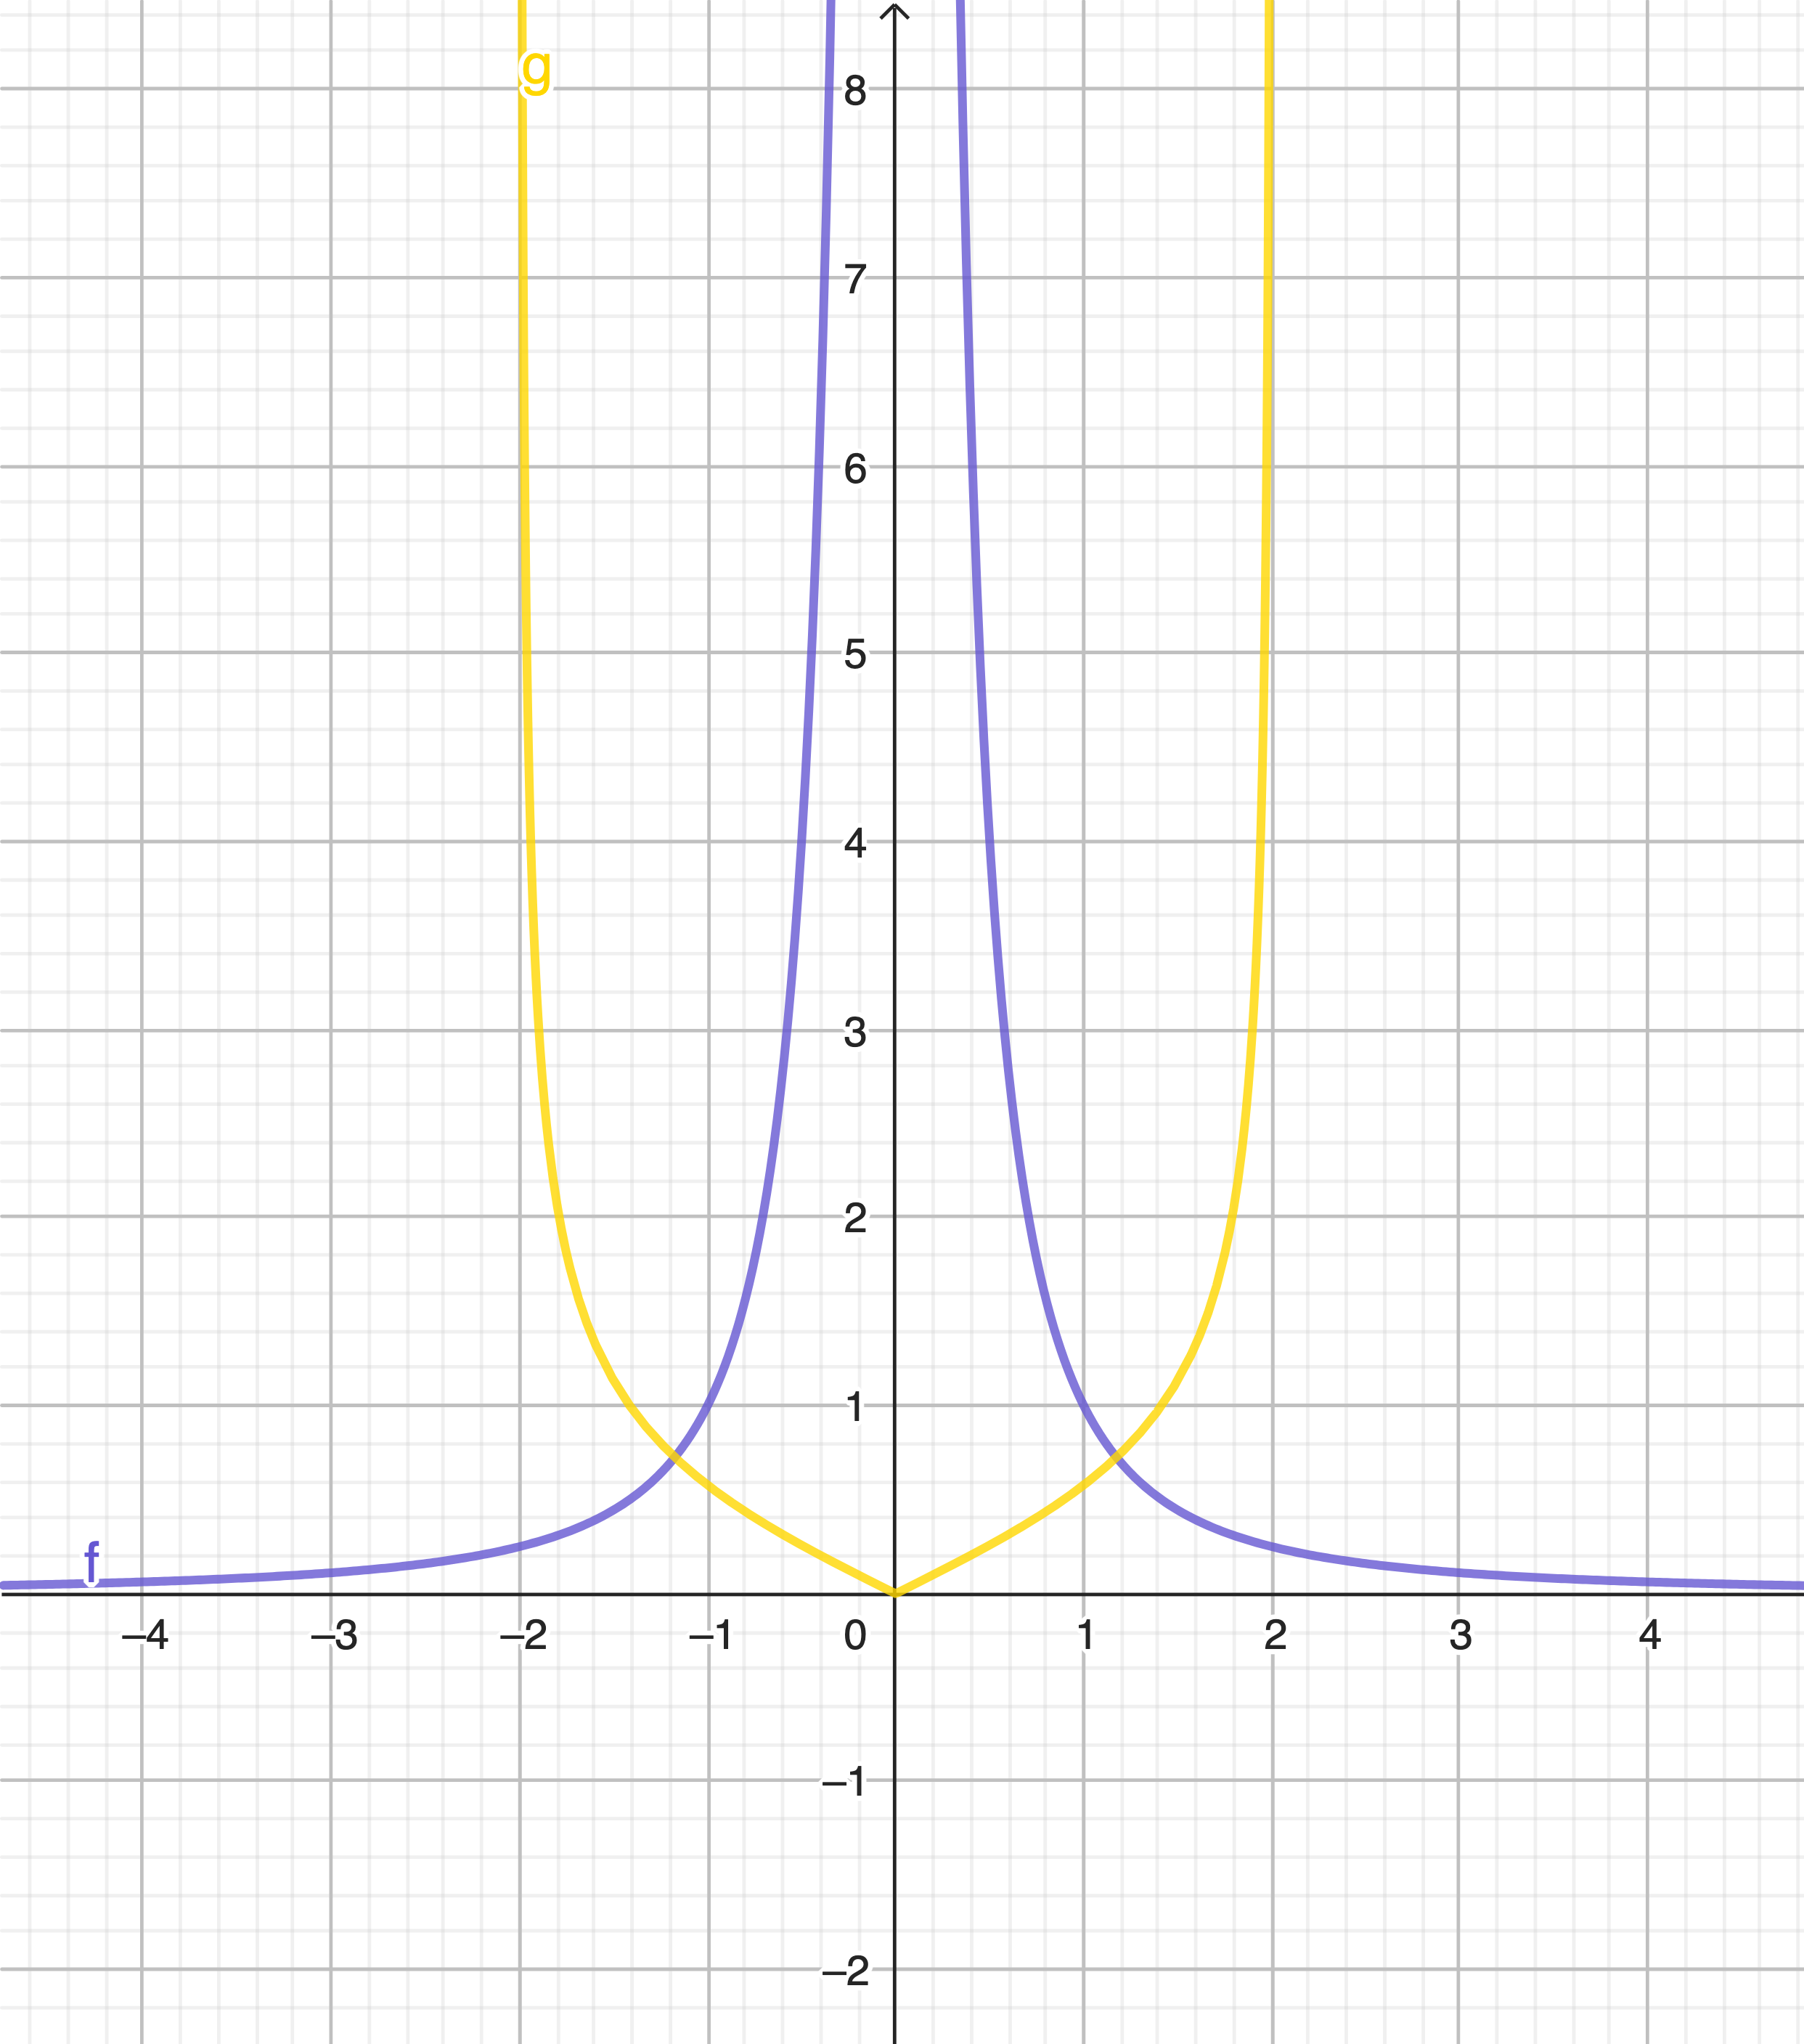
\includegraphics[width=0.6\textwidth]{images/grafico.png}
  \caption{Funzione b (viola) e a (gialla)}
  \label{fig:funzione1}
\end{figure} 
Prendendiamo un intervallo vicino alla soluzione $\overline{S((2,0.7), 0.6)}$.
Quindi avremmo:
\[
\begin{matrix}
1.4\leq x\leq2.6\\
0.1 \leq y \leq 1.3	
\end{matrix}
\]
Prendiamo x minima (a sinistra) e y massima (a destra) rispettivamente quindi $1.4$ e $1.3$. Eseguiamo i calcoli:
\[
\begin{matrix}
	\frac{1}{1.4}\approx0.714&&
	\frac{1.3}{\sqrt{4-1.3^2}}\approx0.855
\end{matrix}
\]
Quindi tornando alla nostra norma della Jacobiana possiamo maggiorare con:
\[
 \frac{|y|}{|\sqrt{4-y^2}|}\leq0.855  \frac{1}{|x^2|}\leq0.714 
\]
Dunque $\max{(0.855,0.714)}=0.855$ che sarà sempre minore uguale a $L$.\\
Vale quindi la L liptchiziana\\
Iniziamo con la prima funzione $a$:\\
Possiamo vedere che la funzione è continua, e monotona crescente nell'intervallo maggiore uguale a 0. Noi di queste funzioni interessa prendere l'area compresa tra l'area  tra le due funzioni nella parte positiva. Quello che ci interessa è il limite destro della funzione in questo caso. Prendiamo la prima degli intervalli che abbiamo trovato precedentemente ovvero $0.1\leq x\leq 1.3$.
Deduciamo quindi che:\\
\[
	\frac{\partial g_2}{\partial x}\leq \frac{\partial g_2}{\partial x}(0.1)
\] e anche
\[
	\frac{\partial g_1}{\partial y}\leq \frac{\partial g_1}{\partial y}(1.3)
\]
Possiamo dunque affermare che non ci sono problemi relativi alla convergenza in questo ambito.
\\Seguiamo con la seconda $b$:\\
Come prima prendiamo l'intervallo maggiore di 0, Possiamo vedere che è una funzione continua monotona decrescente, quindi crescente verso sinistra.\\
Facciamo la stessa cosa precedentemente ma con l'intervallo $1.4\leq y\leq2.6$
Deduciamo quindi che:\\
\[
	\frac{\partial g_2}{\partial x}\leq \frac{\partial g_2}{\partial x}(1.4)
\] e anche
\[
	\frac{\partial g_1}{\partial y}\leq \frac{\partial g_1}{\partial y}(2.6)
\]
Anche qui sono verificate le nostre condizioni. Possiamo quindi affermare che il metodo è ben definito poichè $x^{(k)} \in S(x^*,\rho)$ e il metodo converge sempre
\section*{Pratica}
Per l'iterazione iniziale, si prende:
\[
  x^{(0)} = \begin{bmatrix} 0.1 \\ 0.5 \end{bmatrix}.
\]

La soluzione esatta del sistema, calcolata analiticamente, è:
\[
\begin{cases}
  x = \sqrt{2 + \sqrt{3}} \approx 1.93185, \\
  y = \dfrac{1}{x} \approx 0.51764.
\end{cases}
\]
L'obiettivo è verificare che il metodo converga alla soluzione.

\subsection*{Codice MATLAB per il Metodo di Approssimazione Successiva}

\begin{lstlisting}
close all
clear all
clc

%% Definizione della funzione di iterazione per il sistema
g = @(x) [sqrt(4 - x(2)^2);  % x_{n+1} = sqrt(4 - y_n^2)
          1/x(1)];           % y_{n+1} = 1/x_n

% Soluzione esatta (calcolata analiticamente)
exact_x = sqrt(2 + sqrt(3));   % ~1.93185
exact_y = 1/exact_x;           % ~0.51764
sol = [exact_x; exact_y];

% Parametri di ingresso
x0 = [0; 0.5];  % Guess iniziale vicino alla soluzione
tol = 1e-6;
maxit = 60;

% Chiamata alla funzione di punto fisso
[x, it, iterati] = fixed(g, x0, maxit, tol);

% Calcolo residuo ed errore
fprintf('Iterazioni effettuate: %d \nSoluzione: [%.12f, %.12f]\n', it, x);
for i = 1:it+1
    res(i) = norm(iterati{i} - g(iterati{i})); % Residuo
    err(i) = norm(iterati{i} - sol, inf);      % Errore assoluto
end

% Plot del residuo
figure;
semilogy(1:it+1, res, 'r*-');
title('Residuo vs Iterazioni');
xlabel('Iterazioni'); ylabel('||x_k - g(x_k)||');

% Plot dell'errore
figure;
semilogy(1:it+1, err, 'b*-');
title('Errore assoluto vs Iterazioni');
xlabel('Iterazioni'); ylabel('||x_k - x^*||_{\infty}');

% Stima dell'ordine di convergenza
[p, C] = stima_ordine(iterati); 
fprintf('Ordine stimato: %.3f \t Costante asintotica: %.3f\n', p, C);
\end{lstlisting}

\subsection*{Funzione Fixed Point}

\begin{lstlisting}
function [x,it,iterati]=fixed(g,x0,maxit,tol)
% g     funzione
% x0    punto iniziale
% maxit numero massimo di iterazioni
% tol   tolleranza relativa
%
x = x0;
iterati{1} = x;
for it = 1:maxit
    x1 = feval(g, x);
    iterati{it+1} = x1;
    if norm(x1 - x, inf) < eps + tol * norm(x, inf) % Convergenza raggiunta
        break
    end
    x = x1;  
end
end
\end{lstlisting}

\subsection*{Funzione per la Stima dell'Ordine di Convergenza}

\begin{lstlisting}
function [ordine,stima] = stima_ordine(xvect)
% Stima ordine e costante asintotica di convergenza

nit = length(xvect);
p = zeros(nit-1, 1);  % Vettore degli ordini
c = zeros(nit-1, 1);  % Vettore delle costanti

for i = 3:nit-1
    diff1 = norm(xvect{i+1} - xvect{i});
    diff2 = norm(xvect{i} - xvect{i-1});
    diff3 = norm(xvect{i-1} - xvect{i-2});

    if abs(diff1) <= eps || abs(diff2) <= eps || abs(diff3) <= eps
        p(i) = p(i-1);  % Se la precisione è troppo bassa, manteniamo il valore precedente
        c(i) = c(i-1);
    else
        num = log(diff1 / diff2);
        den = log(diff2 / diff3);
        p(i) = num / den;
        c(i) = diff1 / diff2^p(i);
    end
end
ordine = p(end);
stima = c(end);
end
\end{lstlisting}

\subsection*{Risultati da Console}

Il codice fornisce la soluzione ottenuta, il residuo e l'errore assoluto ad ogni iterazione. Ecco un esempio dei risultati:
\begin{lstlisting}[style=console]
Iterazioni effettuate: 13 	 
Soluzione: [1.931853363035, 0.517638057300]
Ordine stimato: 1.000 	 Costante asintotica: 0.268
\end{lstlisting}

Come si può notare, i risultati sono molto vicini alla soluzione analitica. Il sistema converge dopo 13 iterazioni con velocità lineare (ordine stimato = 1). Se avessimo ottenuto un ordine pari a 2, la convergenza sarebbe stata quadratica (l'errore si ridurrebbe, ad esempio, di un fattore 4 ad ogni iterazione, mentre nel caso lineare si riduce di un fattore 2).

\section*{Esercizio 2}
\textbf{Problema:} Usare il metodo di Newton per risolvere il sistema dell’esercizio precedente. Verificare sperimentalmente che, a partire dal punto \((0.5,2)\), il metodo converga localmente.

\subsection*{Metodo di Newton}
Il metodo di Newton si basa sullo sviluppo in serie di Taylor della funzione e utilizza la derivata (la Jacobiana) della funzione. In generale:
\[
  x^{(k+1)} = x^{(k)} - J(x^{(k)})^{-1} f(x^{(k)}),
\]
dove la matrice Jacobiana \( J(x) \) è definita come:
\[
	J_{ij} = \frac{\partial f_i}{\partial x_j}.
\]

Consideriamo il sistema:
\[
f(x,y)=
\begin{cases}
	x^2 + y^2 - 4,\\[1mm]
	x \cdot y - 1.
\end{cases}
\]
La Jacobiana risulta essere:
\[
J(x,y)=
\begin{pmatrix}
	2x & 2y\\[1mm]
	y & x
\end{pmatrix}.
\]

Per il punto iniziale, si prende:
\[
x^{(0)} = \begin{pmatrix} 2 \\ 0.5 \end{pmatrix}.
\]
L'obiettivo è verificare che il metodo converga alla soluzione.

\subsection*{Codice MATLAB per il Metodo di Newton}

\begin{lstlisting}
close all
clear all
clc

%% Definizione della funzione f e della sua Jacobiana J
f = @(x) [x(1)^2 + x(2)^2 - 4;
          x(1)*x(2) - 1];

J = @(x) [2*x(1), 2*x(2);
          x(2),   x(1)];

% Soluzione esatta (calcolata analiticamente)
exact_x = sqrt(2 + sqrt(3));   % ~1.93185
exact_y = 1/exact_x;           % ~0.51764
sol = [exact_x; exact_y];

% Parametri di ingresso
x0 = [2; 0.5];  % Guess iniziale dato dalla consegna del problema
tolx = 1e-6; tolf = 1e-6;
maxit = 60;

% Chiamata alla funzione Newton
[x, it, iterati] = sis_newton(f, J, x0, tolx, tolf, maxit);

% Calcolo residuo ed errore
fprintf('Iterazioni effettuate: %d \t Soluzione: [%.12f, %.12f]\n', it, x);
for i = 1:it+1
    res(i) = norm(iterati{i} - f(iterati{i})); % Residuo
    err(i) = norm(iterati{i} - sol, inf);      % Errore assoluto
end

% Plot residuo
figure;
semilogy(1:it+1, res, 'r*-');
title('Residuo vs Iterazioni');
xlabel('Iterazioni'); ylabel('||f(x_k)||');

% Plot errore
figure;
semilogy(1:it+1, err, 'b*-');
title('Errore assoluto vs Iterazioni');
xlabel('Iterazioni'); ylabel('||x_k - x^*||_{\infty}');

% Stima ordine di convergenza
[p, C] = stima_ordine(iterati); 
fprintf('Ordine stimato: %.3f \t Costante asintotica: %.3f\n', p, C);
\end{lstlisting}

\subsection*{Funzione Newton}

\begin{lstlisting}
function [x, it, iterati] = sis_newton(fvett, jac, x0, tolx, tolf, maxit)
    x = x0(:);
    iterati{1} = x;
    f_val = feval(fvett, x);
    J_val = feval(jac, x);
    for it = 1:maxit
        dx = J_val \ (-f_val);  % Calcolo dell'incremento
        x = x + dx;
        f_val = feval(fvett, x);
        iterati{it+1} = x;
        if (norm(dx, inf) <= eps + tolx * norm(x, inf)) && (norm(f_val, inf) <= tolf)
            break
        end
        J_val = feval(jac, x);
    end
    if it >= maxit
        fprintf('Raggiunto il massimo numero di iterazioni\n');
    end
end
\end{lstlisting}

\subsection*{Risultati da Console}

Esempio di output ottenuto dalla console:
\begin{lstlisting}[style=console]
Iterazioni effettuate: 3 	 
Soluzione: [1.931851652579, 0.517638090204]
Ordine stimato: 1.933 	 Costante asintotica: 0.313
\end{lstlisting}

Si osserva che il metodo di Newton converge in sole 3 iterazioni e, contrariamente al metodo delle approssimazioni successive, mostra una convergenza di ordine quadratico (il che implica una riduzione dell'errore molto più rapida ad ogni iterazione).

\section*{Differenza tra Es1 e Es2}
Poniamo che entrambi gli esercizi utilizzino le stesse coordinate iniziali
\[
x_0=\begin{pmatrix} 2 \\ 0.5 \end{pmatrix}
\]
e che le tolleranze siano uguali. Di seguito si riportano i risultati grafici.

\begin{figure}[h]
  \centering
  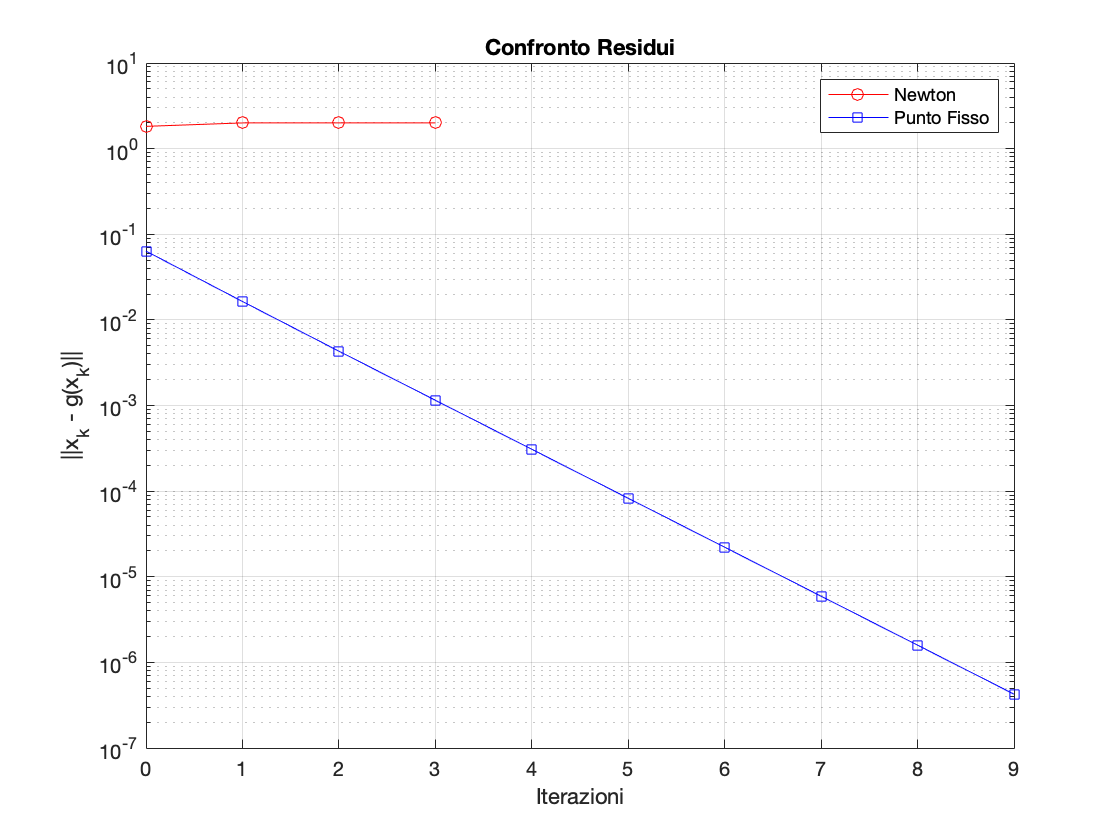
\includegraphics[width=0.7\textwidth]{images/figure1.png} 
  \caption{Confronto dei residui per iterazioni}
  \label{fig:residui}
\end{figure}

Nella figura si osserva come il residuo vari in funzione delle iterazioni. In particolare, il metodo delle approssimazioni successive, pur raggiungendo un residuo minore, richiede un numero maggiore di iterazioni rispetto al metodo di Newton. Quest'ultimo, infatti, converge in 3 iterazioni, mentre il primo impiega circa 9 iterazioni.

\begin{mdframed}[linecolor=blue, linewidth=1pt, roundcorner=10pt]
\paragraph{Esempio Pratico}
Il residuo associato a un sistema lineare \(A\mathbf{x} = \mathbf{b}\) è definito come:
\[
\mathbf{r} = \mathbf{b} - A\mathbf{x},
\]
che rappresenta la differenza tra il termine noto \(\mathbf{b}\) e la stima \(A\mathbf{x}\).
\end{mdframed}

\begin{figure}[h]
  \centering
  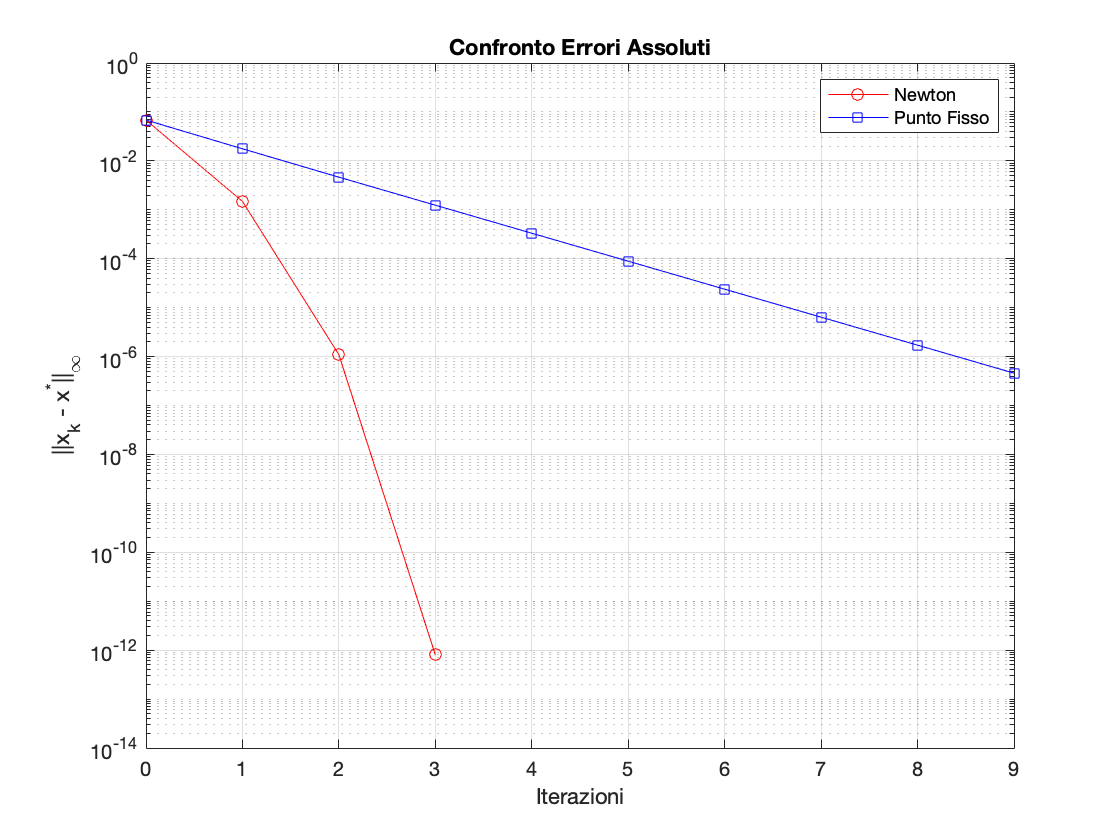
\includegraphics[width=0.7\textwidth]{images/figure2.png} 
  \caption{Confronto degli errori assoluti per iterazioni}
  \label{fig:errore}
\end{figure}

Nel grafico degli errori, si nota come l'errore assoluto nel metodo delle approssimazioni successive sia maggiore rispetto a quello ottenuto con il metodo di Newton, che raggiunge valori prossimi alla tolleranza impostata.

\begin{lstlisting}[style=console]
============= RISULTATI =============
Newton: Ordine 1.933 - Costante 0.313
Punto Fisso: Ordine 1.000 - Costante 0.268	
\end{lstlisting}

Come evidenziato, la velocità di convergenza (cioè la rapidità con cui l'errore si riduce ad ogni iterazione) è significativamente maggiore per il metodo di Newton, confermando la convergenza quadratica rispetto alla convergenza lineare del metodo delle approssimazioni successive.




%%%%%%%%%%%%%%%%%%%%%%%%%%%%%%%%%%%%%%%%%%




\section*{Esercizio 3 (Aereo)}

Si consideri un modello semplificato di controllo della stabilità di un aereo in risposta ai comandi del pilota, basato su equazioni di bilanciamento delle forze, in cui il termine di gravità è ignorato. Si tratta di un sistema di 5 equazioni in 8 incognite, dato da:
\begin{equation*}
  A x + \psi(x) = 0,
\end{equation*}
dove
\begin{equation*}
  A =
  \begin{pmatrix}
    -3.933 & 0.107 & 0.126 & 0     & -9.99  & 0      & -45.83 & -7.64 \\
    0      & -0.987& 0     & -22.95& 9      & -28.37& 0      & 0     \\
    0.002  & 0     & -0.235& 0     & 5.67   & 0      & -0.921 & -6.51 \\
    0      & 1.0   & 0     & -1.0  & 0      & -0.168& 0      & 0     \\
    0      & 0     & -1.0  & 0     & -0.196 & 0      & -0.0071& 0
  \end{pmatrix}
\end{equation*}
e
\begin{equation*}
  \psi(x) =
  \begin{pmatrix}
    -0.727\,x_2x_3 + 8.39\,x_3x_4 - 684.4\,x_4x_5 + 63.5\,x_4x_2 \\
    0.949\,x_1x_3 + 0.173\,x_1x_5 \\
    -0.716\,x_1x_2 - 1.578\,x_1x_4 + 1.132\,x_4x_2 \\
    -x_1x_5 \\
    x_1x_4
  \end{pmatrix}.
\end{equation*}

Le variabili \( x_1, x_2, x_3 \) rappresentano le velocità di rollio, beccheggio e imbardata, mentre \( x_4, x_5 \) sono gli angoli di attacco e di derapata. Le ultime tre variabili \( x_6, x_7, x_8 \) sono i controlli (deviazione di elevatore, alettone, timone).

Per studiare il comportamento dell’aereo al variare dei controlli, per ogni terna delle variabili di controllo, si deve risolvere un sistema di 5 equazioni in 5 incognite.

Nel caso dell’aereo, si consideri la partizione della matrice \( A \) in
\[
A = [A_1 \quad A_2],
\]
con
\[
A_1 \in \mathbb{R}^{5\times5},\quad A_2 \in \mathbb{R}^{5\times3},
\]
e si scriva la variabile \( x \) come
\[
x = \begin{pmatrix} w \\ u \end{pmatrix},\quad w \in \mathbb{R}^{5},\quad u \in \mathbb{R}^{3}.
\]
Per un controllo \( u \) fissato, siccome \( A_1 \) è non singolare, si ha:
\begin{equation*}
  A_1 w + A_2 u + \psi(w) = 0.
\end{equation*}
Pertanto, applicando l'inverso di \( A_1 \) si ottiene:
\begin{equation*}
  w = -A_1^{-1} \Bigl( A_2 u + \psi(w) \Bigr).
\end{equation*}

Dunque vale:
\[
\varphi(x) = A_1^{-1}.
\]

Bene, ora trascrivere il seguente esercizio in MATLAB. Per rendere l'esercizio più carino ho inserito un timer che inizia ad ogni metodo e che ne calcola il tempo di esecuzione. Ho usato 2 metodi. Una risoluzione per sistema e una risoluzione con il metodo delle approssimazioni successive. Ho provato ad usare anche Newton ma quando ho dovuto calcolarmi la Jacobiana del sistema diventava una matrice molto complessa e molto grande. Ho preferito evitare. \\
Poniamo $x0$ come:
\[
x0=\begin{bmatrix}
	0\\0
\end{bmatrix}
\] 
e i comandi del pilota $u$ come:
\[
u=\begin{bmatrix}
	0.1 &0.1 &0.1
\end{bmatrix}
\]
Dove u indica da 0 a 1 le x,y,z nello spazio dove il pilota vuole muoversi.

\section*{Codice MATLAB per il Metodo di Approssimazione Successiva}

Di seguito è riportato il codice MATLAB utilizzato per risolvere l'esercizio dell'aereo:

\begin{lstlisting}
	close all
clear all
clc
addpath("/Users/tobiasacchetto/Documents/GitHub/Numerical_Analysis_II/Function");

A= [
    -3.933 0.107 0.126 0 -9.99 0 -45.83 -7.64;
    0 -0.987 0 -22.95 9 -28.37 0 0;
    0.002 0 -0.235 0 5.67 0 -0.921 -6.51;
    0 1.0 0 -1.0 0 -0.168 0 0;
    0 0 -1.0 0 -0.196 0 -0.0071 0;
    ];

%x1=velocita' di rollio
%x2=velocita' di beccheggio
%x3=velocita' di imbardata
%x4=angolo di attacco
%x5=angolo di derapata
%x6=controlli di deviazione
%x7=controlli di alettone
%x8=controlli di timone
A1=A(1:5,1:5);
A2=A(1:5,6:8);

psi = @(w) [ -0.727*w(2)*w(3) + 8.39*w(3)*w(4) - 684.4*w(4)*w(5) + 63.5*w(4)*w(2);
             0.949*w(1)*w(3) + 0.173*w(1)*w(5);
            -0.716*w(1)*w(2) - 1.578*w(1)*w(4) + 1.132*w(4)*w(2);
            -w(1)*w(5);
             w(1)*w(4) ]; 

% Example control inputs (replace with actual values)
u = [0.1; 0.1; 0.1]; % [x6; x7; x8]

% Initial guess for w (x1 to x5)
w_old = zeros(5, 1);

% Iteration parameters
max_iter = 100;
tolerance = 1e-6;

tic;
% Fixed-point iteration
for iter = 1:max_iter
    psi_w = psi(w_old);
    rhs = A2 * u + psi_w;
    w_new = - (A1 \ rhs);  %sarebbe A1*w^(k+1)=-(A_2*u+psi(w^k))
    
    if norm(w_new - w_old) < tolerance
        fprintf('Convergenza raggiunta in %d iterazioni.\n', iter);
        break;
    end
    w_old = w_new;
end
tempo=toc;
% Output the result
disp('Computed state vector w:');
disp(w_new);
fprintf("Il tempo mio e' %g \n\n",tempo);

f=@(x)(-inv(A1)*(A2*u+psi(x)));
tic;
[x,it,iterati]=fixed(f,w_old,max_iter,tolerance);
tempo=toc;
disp('Computed state vector w:');
disp(x);
fprintf('Numero di iterazioni: %d\n',it);
fprintf("Il tempo e' %g \n\n",tempo);
\end{lstlisting}

\section*{Risultati da Console}
\begin{lstlisting}[style=console]
Convergenza raggiunta in 14 iterazioni.
Computed state vector w:
   -0.0363
   -0.0580
   -0.0237
   -0.0700
    0.1303

Il tempo e' 0.00674418 

Computed state vector w:
   -0.0363
   -0.0580
   -0.0237
   -0.0700
    0.1303

Numero di iterazioni: 3
Il tempo e' 0.00463188 
\end{lstlisting}
Si osserva che, nel primo caso (mediante la messa a sistema delle matrici), la convergenza viene raggiunta dopo 14 iterazioni, mentre nel secondo, usando il metodo delle approssimazioni con \texttt{feval}, il risultato si ottiene in sole 3 iterazioni, evidenziando anche una marcata differenza in termini di tempo di esecuzione. \\
Tuttavia, il sistema risulta instabile: se in input u viene associato un valore per una qualsiasi delle variabili x,y,z superiore a 0.16, il sistema smetterebbe di convergere, rendendolo quindi estremamente instabile
\begin{lstlisting}[style=console]
	Computed state vector w:
   NaN
   NaN
   NaN
   NaN
   NaN

Il tempo e' 0.00438463 

Computed state vector w:
   NaN
   NaN
   NaN
   NaN
   NaN

Numero di iterazioni: 100
Il tempo e' 0.00816623 
\end{lstlisting}

\end{document}
